\part*{Part IV --- The compression limit and the edit method (version 2.2)}
\addcontentsline{toc}{part}{Part IV --- The compression limit and the edit method (version 2.2)}

\section{The compression limit}\label{sec:limit}

Every method of Parts~II and~III reproduces the FDS at one Basquin exponent $b$, the one of the damage
model. This section asks what happens at the other exponents, and arrives at a statement about how far a
record can be shortened at all. The answer is a curve that can be computed from the record alone, before
any synthesis.

\subsection{Damage as a moment of the cycle histogram}\label{sec:mellin}

Fix one oscillator of the grid and collect the rainflow cycles of its response: $N$ cycles with
amplitudes $A_c$ (half cycles count with $n_c = \tfrac12$). Write their distribution as a density $p(A)$,
so that $N p(A)\,\dd A$ is the number of cycles with amplitude in $(A, A+\dd A)$. The
damage~\eqref{eq:minerz} is then
\begin{equation}\label{eq:mellin}
  D_b = \frac{K^b}{C}\sum_c n_c A_c^b = \frac{K^b}{C}\,N\!\int_0^\infty A^b\,p(A)\,\dd A
  = \frac{K^b}{C}\,N\,\E[A^b].
\end{equation}
The damage at exponent $b$ is the $b$-th moment of the cycle-amplitude distribution (in the language of
integral transforms, the Mellin transform of $p$ at $b+1$). The FDS of the damage model is one such
moment per oscillator. Two consequences follow at once.

\begin{result}[The FDS at every exponent is the cycle histogram]
If two signals have the same rainflow cycle distribution at an oscillator (same $N$, same $p$), their
damage is equal for every exponent $b$. Conversely, if their damage is equal for every $b$ in an
interval, the distributions coincide (the moments of a distribution with a light tail, such as the
Rayleigh mixtures of Section~\ref{sec:rice}, determine it). ``Equal FDS for every $b$'' and ``equal
cycle histogram'' are the same statement.
\end{result}

This is the reason to care about other exponents: the exponent of a real component is uncertain
(material, weld class and surface change it), and a test that is right for every $b$ does not depend
on that uncertainty. It is also a description independent of Miner's rule, usable with any damage
model that is a function of the cycle amplitudes.

\subsection{Why a shorter test cannot be exact for every exponent}\label{sec:bzero}

Let a test profile be built from the record with an amplitude factor $\lambda$ and the duration
$T/\alpha$. Let $N_t$ and $N_r$ be the numbers of cycles of the test and of the record at an
oscillator, and $\E_t$, $\E_r$ the averages over their cycles. Equal damage for every $b$ requires
\begin{equation}
  \lambda^b\,N_t\,\E_t[A^b] = N_r\,\E_r[A^b]\qquad\text{for every } b .
\end{equation}
Set $b=0$: $\lambda^0 = 1$ and $\E[A^0] = 1$, so $N_t = N_r$. But the cycles of a narrow-band response
arrive at the rate of the natural frequency (one per period, Section~\ref{sec:rice}), so a test of
duration $T/\alpha$ holds about $N_r/\alpha$ cycles. The two statements are compatible only for
$\alpha = 1$.

\begin{result}[No scaling is exact for every exponent]
A profile obtained by scaling a shorter signal cannot reproduce the damage of the record at every
exponent, because the moment of order zero, the number of cycles, is reduced by the compression.
\end{result}

The way out is in the same equation. The small cycles make up most of the count, but at a large
exponent they contribute almost nothing to the damage. If a shorter test drops exactly the small cycles
and keeps the large ones, the number of cycles changes (the zero-order moment is lost) while the high
moments are preserved. On a time history there is one operation that does this: keep the stretches of
the record that carry the damage, unchanged, and leave out the quiet ones. Section~\ref{sec:edit}
builds a method on it. How far it can go is the question of the next subsection.

The error of dropping the cycles below an amplitude $A_0$ is the share of the damage they carry,
\begin{equation}
  \varepsilon_b = \frac{\int_0^{A_0} A^b p(A)\,\dd A}{\int_0^\infty A^b p(A)\,\dd A},
\end{equation}
which decreases with $b$. For a Rayleigh distribution and $A_0 = \sigma_z$ (which discards 39\,\% of
the cycles), the substitution of~\eqref{eq:rayleighmoment} gives the regularised incomplete Gamma
function $P(1+b/2,\,\tfrac12)$: $\varepsilon_3 = 0.037$, $\varepsilon_5 = 0.005$, $\varepsilon_9 =
0.0001$. A large exponent does not notice the loss; a small one does, which is why an edited test is
below the record at $b = 3$ in the tables of Section~\ref{sec:editresults}.

\subsection{The damage Lorenz curve}\label{sec:lorenz}

Cut the record into consecutive windows of length $L_w$ (Section~\ref{sec:editwindows} says how $L_w$
is chosen) and compute, for every oscillator $i$ of the grid, the share $W_{ij}$ of its damage that
falls in window $j$: the rainflow damage of the response in that window, divided by the damage over
the whole record. Every row of $W$ sums to 1. Sort the windows from the most to the least valuable (the
ranking is defined in Section~\ref{sec:ranking}) and add up the shares along the ranking.

\begin{result}[Damage Lorenz curve and compression limit]
Let $q$ be the fraction of the time kept (the first $qM$ windows of the ranking, out of $M$) and
$L_i(q)$ the share of the damage of oscillator $i$ contained in them. $L_i$ is the damage Lorenz curve
of the oscillator: $L_i(0) = 0$, $L_i(1) = 1$, non-decreasing and concave, and equal to the diagonal
$L(q) = q$ when the damage is spread uniformly over the time. The curve of the worst-served
oscillator, $L_{\min}(q) = \min_i L_i(q)$, sets the compression limit: the largest time compression
at which editing alone keeps a share $\rho$ of the damage at every oscillator is
\begin{equation}\label{eq:alphamax}
  \alpha_{\max}(\rho) = \frac{1}{q(\rho)},\qquad L_{\min}\bigl(q(\rho)\bigr) = \rho .
\end{equation}
\end{result}

Three properties follow from the definition. The curve lies higher the more the damage is concentrated
in time: a stationary Gaussian record has the diagonal and cannot be shortened by editing at all, a
record with bursts can. It also rises with $b$, because a larger exponent concentrates the damage in
fewer cycles: a large exponent allows more compression. And it is different for every oscillator: the
damage of a low-frequency oscillator excited by a few shocks sits in a few windows, that of an
oscillator driven by a stationary band is spread out. A test has to be right at every natural frequency,
so the binding curve is $L_{\min}$, not the mean over the oscillators (which the interface shows as
well, because it tells how much is lost on average).

Beyond $\alpha_{\max}$ the record has no more quiet time to drop. The remaining compression can only come
from raising the amplitude, and with it the dependence on the exponent returns, because an amplitude
factor acts as its $b$-th power on the damage. The two mechanisms are therefore not competitors but
two stages: editing up to the limit, amplitude beyond it, with the dependence on $b$ confined to the
part the amplitude did. A test specification is described by the pair, not by $\alpha$ alone.

\begin{figure}[htb]\centering
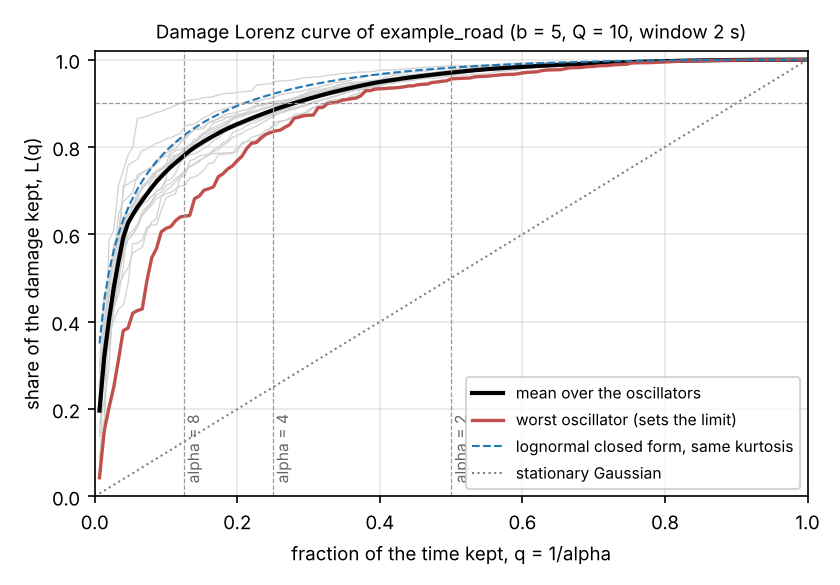
\includegraphics[width=0.62\textwidth]{figures/lorenz_example_road.png}
\caption{Damage Lorenz curves of the example record (grey: one curve per oscillator). Keeping the most
damaging quarter of the time keeps 88\,\% of the damage on average and 82\,\% at the worst oscillator;
the 90\,\% limit is $\alpha_{\max} = 3.0$. The dashed curve is the closed form of
Section~\ref{sec:lognormal} for the kurtosis of the record.}
\label{fig:lorenz}
\end{figure}

\subsection{Closed form for a lognormal envelope}\label{sec:lognormal}

The Lorenz curve of a modulated Gaussian signal $x = e\,g$ (Section~\ref{sec:modulated}) can be written
in closed form when the local variance $s = e^2\sigma_g^2$ is lognormal. The result is useful as an
estimate before any computation and as a reference against which a measured curve is compared.

Let $s = e^{Y}$ with $Y$ Gaussian of mean $\mu$ and standard deviation $\tau$. By
Section~\ref{sec:kzdamage} the damage of a stretch of time with local variance $s$ is proportional to
$s^{b/2}$, so the damage share of the stretches with $Y > y_0$ is $\E[s^{b/2}\mathbf 1_{Y>y_0}]
/ \E[s^{b/2}]$, and their time share is $q = P(Y > y_0)$. Two facts about Gaussian variables are
needed. First, $P(Y > y_0) = \Phi(u)$ with $u = (\mu - y_0)/\tau$ and $\Phi$ the standard normal
distribution function. Second, the truncated expectation of an exponential of $Y$: writing $c = b/2$,
\begin{equation}
  \E\bigl[e^{cY}\mathbf 1_{Y>y_0}\bigr] = \int_{y_0}^\infty e^{cy}\,\frac{1}{\tau\sqrt{2\pi}}
  e^{-(y-\mu)^2/(2\tau^2)}\,\dd y .
\end{equation}
Completing the square in the exponent, $cy - \frac{(y-\mu)^2}{2\tau^2} = c\mu + \frac{c^2\tau^2}{2}
- \frac{(y-\mu-c\tau^2)^2}{2\tau^2}$, the integrand becomes a Gaussian density centred at
$\mu + c\tau^2$ times the constant $e^{c\mu + c^2\tau^2/2} = \E[e^{cY}]$, so
\begin{equation}
  \E\bigl[e^{cY}\mathbf 1_{Y>y_0}\bigr] = \E[e^{cY}]\;\Phi\!\left(\frac{\mu + c\tau^2 - y_0}{\tau}\right)
  = \E[s^{b/2}]\;\Phi\!\left(u + \frac{b\tau}{2}\right).
\end{equation}
Dividing by $\E[s^{b/2}]$ and eliminating $u = \Phi^{-1}(q)$:
\begin{result}[Lorenz curve of a lognormal envelope]
\begin{equation}\label{eq:lognlorenz}
  L(q) = \Phi\!\left(\Phi^{-1}(q) + \frac{b\,\tau}{2}\right),\qquad
  \tau = \sqrt{\ln(\kappa/3)},\qquad
  \alpha_{\max}(\rho) = \frac{1}{\Phi\!\left(\Phi^{-1}(\rho) - b\tau/2\right)} .
\end{equation}
\end{result}
The expression of $\tau$ comes from~\eqref{eq:kmod}: for a lognormal $s$, $\tavg{s^2}/\tavg{s}^2 =
e^{\tau^2}$ (the same completion of the square with $c = 2$ and $c = 1$), so $\kappa = 3e^{\tau^2}$.
The whole curve is set by the single number $b\tau/2$: the burstier the record (larger $\kappa$) or the
larger the exponent, the higher the curve.

\begin{center}
\begin{tabular}{lcccccc}
\toprule
& \multicolumn{2}{c}{$b = 5$} & \multicolumn{2}{c}{$b = 7$} & \multicolumn{2}{c}{kurtosis of the edited record} \\
kurtosis $\kappa$ of the record & $\rho = 90\,\%$ & $95\,\%$ & $90\,\%$ & $95\,\%$ & $\alpha = 2$ & $\alpha = 4$ \\
\midrule
4 & 2.1 & 1.6 & 3.6 & 2.5 & 3.5 & 3.3 \\
6 & 4.7 & 3.0 & 19.5 & 9.8 & 4.5 & 4.0 \\
9 & 11.1 & 6.1 & 118 & 47 & 6.1 & 5.0 \\
\bottomrule
\end{tabular}
\end{center}

\noindent\emph{Table 12.1: $\alpha_{\max}$ of~\eqref{eq:lognlorenz} and the kurtosis of the edited record
(Section~\ref{sec:compressedk}) for a lognormal envelope.} The large numbers at $b = 7$ are a warning as
much as a result: the lognormal tail is heavy, and the closed form assumes one envelope common to all
bands. On the example record, whose modulation is nearly common, the formula predicts 98, 92 and
82\,\% of the damage kept at $\alpha = 2$, 4 and 8, and the measured curves give 97, 88 and 79. On the
thesis reference record, where the modulation depends on frequency (Section~\ref{sec:mixturekurt}),
the formula predicts 94\,\% at $\alpha = 4$ against a measured 77\,\% on average and much less at the
worst oscillator. The closed form is an upper estimate; the measured curve of the worst oscillator is the
limit.

\subsection{What the kurtosis of the record says, and what it does not}\label{sec:mixturekurt}

Equation~\eqref{eq:kmod} gives the kurtosis of a modulated signal from its local variance,
$\kappa = 3\tavg{s^2}/\tavg{s}^2$. Turned around, it is a test of the model: estimate $s(t)$ from the
record (the running variance over short windows), form $3\tavg{s^2}/\tavg{s}^2$, and compare it with
the kurtosis measured directly on the samples. If the two agree, the non-Gaussianity of the record is of
the slow-modulation kind, one envelope common to all bands, and the closed form above applies. If the
estimate from the local variance is clearly larger than the direct kurtosis, the bands are not
modulated together: a strong stationary band dilutes the direct kurtosis while the shocks that modulate
the other bands dominate the running variance. This is the situation of Section~\ref{sec:mmvsdmodel},
and it has two consequences for compression: a common envelope (kFDS, or the closed form) cannot
describe the record, and the compression limit is stricter, because the stationary bands have a Lorenz
curve close to the diagonal.

The running variance is itself a random estimate (Appendix~\ref{app:quoted}, C.3), so even a stationary
Gaussian record gives an estimate above 3. The program removes this bias by computing the same estimate
on a phase-randomised copy of the record (same PSD, no modulation) and subtracting its excess over 3.
On the example record the corrected estimate is 6.10 against a direct kurtosis of 6.04; on the thesis
reference record 7.8 against 6.5, and on seven channels of an industrial measurement (not distributed)
the estimate exceeds the direct kurtosis by 0.4 to 1.9 in every channel. Real records are rarely
modulated by one envelope. Their compression limits at 90\,\% retention were between 1.3 and 2.1 at the
worst oscillator, against 3.0 for the example record.
